%%%%%%%%Bilecik �eyh Edebali �niversitesi M�hendsilik Fak�ltesi%%%% 
%%%%%%%%Bilgisayar M�hendisli�i Bitirme �al��mas�%%%%%%%%%%%%%%%%%%
%%%%%%%%%%%%%%%%%%%%%%LaTeX Class%%%%%%%%%%%%%%%%%%%%%%%%%%%%%%%%%%
\documentclass{BUB}
%%%%%%%%%%%%%%%%%%%%%%%%%%%%%%%%%%%%%%%%%%%%%%%%%%%%%%%%%%%%%%%%%%%%%%%%%%%
\begin{document}
\shorthandoff{=}%grafik komutlar�nda babelden kaynaklanan hatay� engeller.
%%%%%%%%%%%%%%%%%%%%%%Bitirme �al��mas�n�n B�l�mleri%%%%%%%%%%%%%%%%%%%%%%%
\thispagestyle{empty}
\begin{figure}[H]
\centering

\includegraphics[scale=0.2]{logomuz}
\end{figure}

\begin{center}
\textbf{T.C.}\\
\textbf{B�LEC�K �EYH EDEBAL� �N�VERS�TES�}\\
\textbf{M�HEND�SL�K FAK�LTES�}

\textbf{B�LG�SAYAR M�HEND�SL��� B�L�M�}
\end{center}
\vfill
\begin{center}
\textbf{RC4 ALGOR�TMASI �LE MET�N VE G�R�NT� ��FRELEME}

\textbf{F�rat U�AR}

\textbf{B�T�RME �ALI�MASI}
\end{center}
\vfill
\begin{center}
\textbf{DANI�MANI : Do�. Dr. Cihan KARAKUZU}

\textbf{B�LEC�K}\\ 
\textbf{\today}
\end{center}


\thispagestyle{empty}
\begin{figure}[H]
\centering

\includegraphics[scale=0.2]{logomuz}
\end{figure}
\begin{center}
\textbf{T.C.}\\
\textbf{B�LEC�K �EYH EDEBAL� �N�VERS�TES�}\\
\textbf{M�HEND�SL�K FAK�LTES�}

\textbf{B�LG�SAYAR M�HEND�SL��� B�L�M�}
\end{center}
\vfill
\begin{center}
\textbf{RC4 ALGOR�TMASI �LE MET�N VE G�R�NT� ��FRELEME}

\textbf{F�rat U�AR}

\textbf{B�T�RME �ALI�MASI}
\end{center}
\vfill
\begin{center}
\textbf{DANI�MANI : Do�. Dr. Cihan KARAKUZU}

\textbf{B�LEC�K}\\ 
\textbf{\today}
\end{center}

\pagenumbering{roman}%romen rakamlar� kullan�lmaya ba�lan�yor.
\setcounter{page}{2}% sayfa numaras�n� ii'den ba�lat�l�yor.
\begin{center}
\textbf{B�LD�R�M}
\end{center}
\begin{singlespace}%1 sat�r aral���
Bu kitaptaki b�t�n bilgilerin etik davran�� ve akademik kurallar �er�evesinde elde edildi�ini ve yaz�m kurallar�na uygun olarak haz�rlanan bu �al��mada bana ait olmayan her t�rl� ifade ve bilginin kayna��na eksiksiz at�f yap�ld���n� bildiririm.
\end{singlespace}
\vspace{2cm}

\begin{center}
\textbf{DECLARATION}
\end{center}
\begin{singlespace}
I hereby declare that all information in this document has been obtained and presented in accordance with academic rules and ethical conduct. I also declare that, as required by these rules and conduct, I have fully cited and referenced all materials and results that are not original to this work.
\end{singlespace}

\vspace{3cm}
\begin{flushright}
\begin{minipage}{5cm}
\begin{center}
\textbf{�mza}
\end{center}
\textbf{��rencinin Ad� SOYADI}

\textbf{Tarih:}\hfill
\end{minipage}
\end{flushright}

\begin{center}
{\bf{\large �ZET}\vspace*{.5cm}

B�T�RME �ALI�MASI

RC4 ALGOR�TMASI �LE MET�N VE G�R�NT� ��FRELEME

F�rat U�AR}

\begin{singlespace}
{\bfseries
Bilecik �eyh Edebali �niversitesi\\
M�hendislik Fak�ltesi\\
Bilgisayar M�hendisli�i B�l�m�}
\end{singlespace}

{\bf Dan��man: Do�. Dr. Cihan KARAKUZU}

{\bf \the\year, \ref{TotPages} Sayfa}

\begin{tabular}{p{7cm}p{2cm}p{4cm}}
\center\textbf{J�ri\; �yeleri}&&\center\textbf{�mza}\cr
\dotfill&&\dotfill\\
\dotfill&&\dotfill\\
\dotfill&&\dotfill
\end{tabular}
\end{center}
{\small  \paragraph{}   RC4 , 1987 y�l�nda Ron Rivest taraf�ndan geli�tirildi. O zamandan beri �e�itli uygulamalarda kullan�lmaktad�r. ARC4 ve ya ARCFOUR olarak da bilinir. RC4 bir ak�� �ifreleme uygulamas�d�r. SSL, WEP,  WPA gibi bir�ok g�ncel uygulamada kullan�lmaktad�r.
 \mbox{} }
 {\paragraph{} RC4 rasgele olarak �retti�i anahtar ak��lar�n�, hem �ifreleme hem de a�ma i�lemi s�ras�nda �zel ve ya i�lemi ile mesaja uygulamaktad�r. Bu projede , RC4 ile metin ve g�r�nt� �ifrelenmektedir. G�r�nt� �ifrelenmeden �nce 2B Cat Map Kaotik Sistemi ile kar��t�r�lmaktad�r. G�r�nt� kar��t�r�ld�ktan sonra RC4 ile �ifrelenmektedir. Ayn� zamanda bu projede, �ifrelenen metin ve g�r�nt�ler RC4 kullan�larak geri d�nd�r�lebilir. \cite{k:1} 
\mbox{}}

{\small \textbf{Anahtar Kelimeler:}  
Cat Map, G�r�nt�, Kaotik, Metin, RC4, �ifreleme}
%%%%%%%%%%%%%%%%%%%%%%%%%%%%%%%%%%%%%%%%%%%%%%%%%%%%%%%%%%%%%%%%%%%%%%%%%%%%%%%%%%%%%%%%%
\newpage
\begin{center}
{\bf{\large ABSTRACT}\vspace*{.5cm}

THESIS

TEXT AND IMAGE ENCRYPTION WITH RC4 ALGORITHM

F�rat UCAR}

\begin{singlespace}
{\bf
Bilecik �eyh Edebali University\\
Engineering Faculty\\
Department of Computer Engineering}
\end{singlespace}

{\bf Advisor: Do�. Dr. Cihan KARAKUZU

\the\year, \ref{TotPages} Pages}

\begin{tabular}{p{7cm}p{2cm}p{4cm}}
\center \textbf{Jury}&&\center \textbf{Sign}\cr
\dotfill& &\dotfill\\
\dotfill& &\dotfill\\
\dotfill& &\dotfill
\end{tabular}
\end{center}
{\small \paragraph{} RC4 was developed in 1987 by Ron Rivest. It is been used in a variety of applications since then. Also known as ARC4 or ARCFOUR. RC4 is a stream encryption application. It is used in many current applications such as SSL, WEP, WPA.
\mbox{}
\paragraph{} RC4 applies randomly generated key flows to the message either during encryption or decompression by xor operation. In this project, text and image are encrypted with RC4. Before the image is encrypted, mixed with 2B Cat Map Chaotic System.After that, image is encrypted with RC4. At the same time in this project, encrypted texts and images can be recalled using RC4. \cite{k:1}
\mbox{}}

{\small \textbf{Keywords:} Cat Map, Chaotic, Encryption, Image, RC4, Text}

\addcontentsline{toc}{section}{�NS�Z}
\section*{�NS�Z}
Bitirme �al��mam�n ba��ndan sonuna kadar eme�i ge�en ve beni bu konuya y�nlendiren sayg� de�er hocalar�m ve dan��man�m Say�n Do�. Dr. Cihan KARAKUZU'ya ve Ar�. G�r. Sefa TUN�ER'e t�m katk�lar�ndan ve hi� eksiltmedikleri desteklerinden dolay� te�ekk�r ederim.

\begin{flushright}
\textbf{F�rat U�AR}

\today
\end{flushright}
%%%��indekiler ve tablolar%%%%%%%%%%%%%%
%%%%%%%%%%%%%%%%%%%%%%���NDEK�LER%%%%%%%%%%%%%
\tableofcontents
%%%%%%%%%%%%%%%%�EK�LLER TABLOSU%%%%%%%%%%%%%%
\renewcommand*\listfigurename{\centerline{\normalsize �EK�LLER TABLOSU}}
\listoffigures%bu komutun oldu�u yerde �ekiller listesi olu�turulur
\addcontentsline{toc}{section}{\normalsize �EK�LLER TABLOSU}
%%%%%%%%%%%%%%%%%%%%%%��ZELGELER TABLOSU%%%%%%%%%%%%%%%%%
\renewcommand*\listtablename{\centerline{\normalsize ��ZELGELER TABLOSU}}
\listoftables%bu komutun oldu�u yerde tablolar listesi olu�turulur
\addcontentsline{toc}{section}{��ZELGELER TABLOSU}
%%%%%%%%%%%%%%%%%%%%%��ZELGELER TABLOSU%%%%%%%%%%%%%%%%%
\textbf{\centerline{KISALTMALAR}}
\addcontentsline{toc}{section}{KISALTMALAR}

\begin{tabular}{l@{ : }l}

\textbf{2B} & 2 Boyut \\
\textbf{CLR} & Ortak Dil �al��mas� \\
\textbf{CRC} & D�ng�sel Art�kl�k Kontrol� \\
\textbf{DES} & Veri �ifreleme Standard� \\
\textbf{DLL} & Dinamik Ba�lant� K�t�phanesi \\
\textbf{ICV} & B�t�nl�k Kontrol De�eri \\
\textbf{IEEE} & Elektrik ve Elektronik M�hendisleri Enstit�s� \\
\textbf{KSA} & Anahtar Planlama Algoritmas� \\
\textbf{LAN} & Yerel Alan A�� \\
\textbf{MIC} & Mesaj B�t�nl��� Kodu \\
\textbf{MSIL} & Microsoft Ara Dili \\
\textbf{PRGA} & Sahte Rasgele �retim Algoritmas�\\
\textbf{SSL} & G�venli Oturum Katman� \\
\textbf{TKIP} & Ge�ici Anahtar B�t�nl��� Protokol� \\
\textbf{WEP} & Kablosuz Denk Mahremiyet \\ 
\textbf{WLAN} & Kablosuz Yerel Alan A�� \\
\textbf{WPA} & Kablosuz Korumal� Eri�im
\end{tabular}
 


\pagenumbering{arabic}%Sayfa numaralamas�n� arap rakamlar�yla yapar.
\setcounter{page}{1}%sayfa numaras�n� 1'den ba�lat�r.
\section{G�R��}
Kriptoloji, saklanmas� veya g�nderilmesi gereken mesajlar�n, bilgilerin bir anahtarla belirli bir sisteme g�re �ifrelenmesi, �ifrelenen mesaj�n anahtar� kullan�larak al�c� taraf�ndan de�ifre edilmesidir. K�saca �ifre bilimine kriptoloji denilmektedir. Kriptografi ve kripto analiz olmak �zere iki dala ayr�l�r. G�n�m�zde teknoloji �ok h�zl� geli�ti�inden g�venlik sorunlar�n� da beraberinde getirmektedir. �zel �irketler, askeri kurumlar, devlet kurumlar� vb. bir�ok birim aras�ndaki ileti�imin g�venli�ini sa�lamak i�in kriptoloji alan�ndaki geli�meler b�y�k �nem arz etmektedir. Bu ama�la g�venlik zaafiyetlerini engellemek ve bunu yaparken h�zl� ileti�imi de sa�lamak amac�yla bir�ok kriptografik y�ntem geli�tirilmektedir. \cite{k:2} 
\begin{figure}[H]
\centering
\scalebox{1}{

\includegraphics[width=10.5cm,height=4.7cm]{kripto}}
\caption{Kriptografi}
\end{figure}
Kriptografik algoritmalar gizlilik, b�t�nl�k, s�reklilik, kimlik denetimi, inkar edilememezlik ve izlenebilirlik gibi g�venlik protokollerinin bile�enleri haberle�mede g�venli�i sa�lamak amac�yla kullan�l�rlar. Kriptografik sistemler simetrik anahtarl�, asimetrik anahtarl� olmak �zere ikiye ayr�l�r fakat anahtars�z �ifrelemede mevcuttur. Simetrik sistemlerde bir gizli anahtar mevcuttur, bu anahtar�n g�nderici ve al�c� tarafta bulunmas� gerekmektedir. Asimetrik sistemlerde gizli bir anahtara ek olarak, a��k anahtar mevcuttur. Bu sistemlerde a��k anahtar ve gizli anahtar�n ikisi ele ge�irildi�inde �ifre ��zme i�lemini yapmak m�mk�nd�r. Bu sayede, a��k anahtar�n ���nc� bir �ah�s taraf�ndan ele ge�irilmesi �ifrelenen bilgilerin ele ge�irilmesi a��s�ndan bir tehdit olu�turmamaktad�r. 
\newpage
Kaos teorisi sonu�lar� tahmin edilemeyen sistemleri a��klayan bilimsel bir ilkedir. Genel anlamda 1980'li y�llarda ara�t�r�lm��t�r. Bir sigara duman�n�n havada yapt��� �ekiller d�zensiz ve ba��ms�z de�ildir. Sigaran�n bu dinamikleri ortamdaki bir�ok etkene ve parametreye ba�l�d�r. Ancak bu parametre ve bilgiler �ok fazlad�r ve bunlar� inceleyip net olarak bir kan�ya varmak imkans�zd�r. Sigara duman�n�n �eklini bulunan ortamdaki r�zgar, s�cakl�k, bas�n� gibi fiziksel b�y�kl�kler etkileyebilir ve bu fakt�rlerin birbirine ba�l� olabilece�i de hesaba kat�ld���nda durum tahmin edilemeyen bir hale gelir. 

Kaotik sistemlerin belirli bir frekans aral���nda bulundu�u ve bu s�n�rlar i�erisinde hareketlerinin belirlenemez oldu�u Lorenz taraf�ndan saptanm��t�r. Kaotik sistemleri, belirli bir alana �eken bu yap�lara kaotik �ekerler ad� verilmektedir. Bu �ekerlere bak�ld���nda bu �ekerleri meydana getiren e�rilerin, belirli say�daki parametreler dizisinin, zaman d�zleminde hi�bir zaman iki kez ayn� rotay� izlemedi�i ve bu rotalar aras�nda kesinlikle k���k de olsa bir farkl�l�k oldu�u g�r�lm��t�r. �ekerlerin olu�turdu�u e�rilerin bu �zelli�inden dolay� fraktal yap�da oldu�u s�ylenebilir. 

Kaotik sistemler g�r�nt� �ifreleme uygulamalar�nda olduk�a yo�un kullan�lmaktad�r. Bilinen kaotik sistemlerin kullan�ld��� ve ba�ar�m ve g�venlik bak�m�ndan olduk�a iyi sonu�lar elde edildi�i g�r�lmektedir. Ayr�ca birden fazla kaotik sistem kullan�lmas� bu sistemlerin ba�lang�� de�erlerine hassas ba�l�l��� ve �ifrelemede kullan�lan parametrelerin fazla olmas� g�venlik seviyesini olduk�a artt�rmaktad�r. Bu sayede �ifrelenen g�r�nt�n�n istenmeyen �ah�slar taraf�ndan ele ge�irilmesi, �ifrelemede kullan�lan parametreleri bilmedi�i taktirde, neredeyse imkans�z hale gelmektedir. 

G�r�nt� �ifrelemede kaotik sistemlerin kullan�lmas�, sa�lad��� baz� �st�nl�klerden ve analiz y�ntemlerine kar�� g�sterdi�i y�ksek dayan�kl�ktan kaynaklanmaktad�r. Bu analizler anahtar g�venli�i, histogram analizi, anahtar hassasl���, g�r�nt�deki biti�ik piksellerin birbiri ile olan ili�ki katsay�s�, bilginin d�zensizlik analizi, �ifreleme ve �ifre ��zme h�z�d�r. Bu sayede, yap�lan her analize kar�� do�rudan daha ba�ar�l� oldu�u s�ylenemese de, genel anlamda kullan�lan geleneksel simetrik ve asimetrik �ifreleme algoritmalar�na kar�� �st�nl�k sa�lad��� g�r�lmektedir. 
  

RC4; SSL, WEP, WPA, gibi g�ncel pek�ok uygulamada kullan�lan bir ak�� �ifreleme uygulamas�d�r. RC4 '�n genel olarak kullan�lan algoritmas� �ekil \ref{1}'deki gibidir. \cite{k:1}

\begin{figure}[H]
\centering
\scalebox{1}{
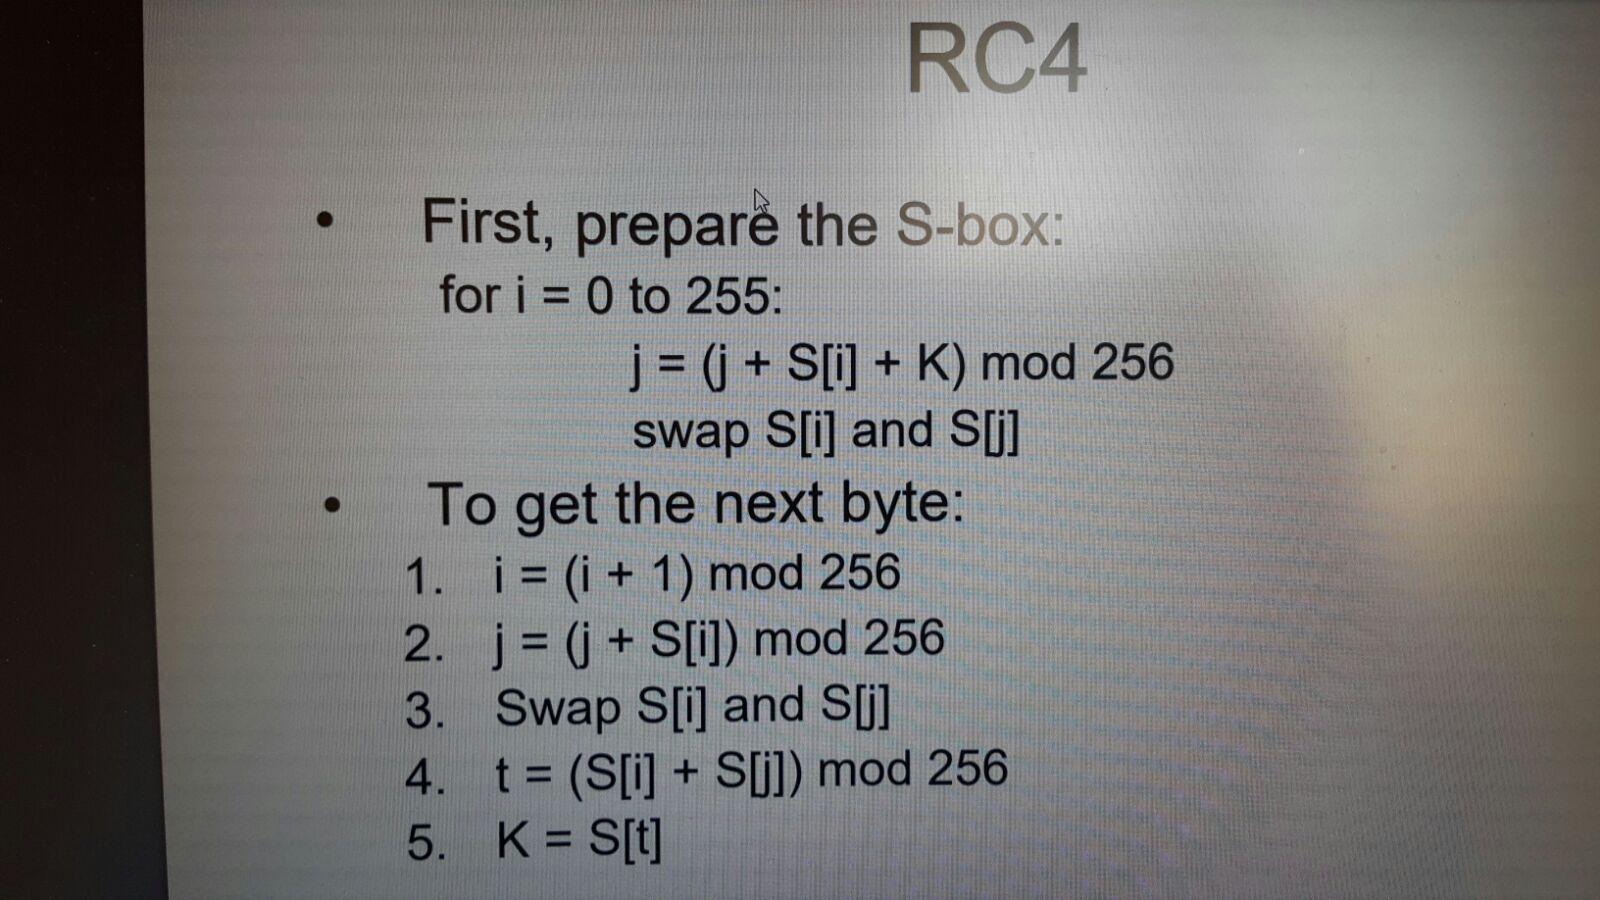
\includegraphics[width=10.5cm,height=6cm]{RC} }
\caption{RC4 algoritmas�}
\label{1}
\end{figure}

Projede metin ve ya g�r�nt� se�imine g�re se�ilen belge RC4 ile �ifrelendi. Bu �ifreleme i�lemi ger�ekle�tirilirken se�ilen belgenin g�r�nt� olmas� durumunda �nce Cat Map ile kar��t�r�ld� ve ard�ndan RC4 uyguland�. Cat Map ile g�r�nt�n�n kar��t�r�lmas� i�lemi ileriki b�l�mlerde detayl� bir �ekilde anlat�lm��t�r. 

RC4 ile �ifreleme i�leme yap�l�rken bir tak�m gereksinimler vard�r. Bunlardan bir tanesi kullan�c� taraf�ndan bir anahtar girilmesidir. Bu �art �ifreleme i�in olmazsa olmaz bir kurald�r. ��nk� �ifreleme i�lemleri yap�l�rken bu girilen anahtar kullan�larak di�er b�l�mlerde detayl� bir �ekilde anlat�lacak olan baz� i�lemler yap�lacakt�r. Bu i�lemler KSA ve PRGA'd�r. Bu iki ad�m�n detayl� anlat�mlar� ve kod k�s�mlar� ilerleyen b�l�mlerde anlat�lacakt�r.

KSA ve PRGA ad�mlar� yap�ld�ktan sonra se�ilen belgenin tipine g�re gerekli i�lemler yap�ld�ktan sonra �ifreleme i�lemi ger�ekle�tirilecektir.


\section{PROGRAMLAMA}
Projede g�r�nt�n�n kar��t�r�lmas� a�amas�nda MATLAB , �ifrelenmesi a�amas�nda ise C\# programlar� kullan�ld�. A�a��da MATLAB ve C\# programlar�n�n ne olduklar� ve kullan�m alanlar� verilmi�tir. 
\subsection{Matlab}
MATLAB temel olarak n�merik hesaplama, grafiksel veri g�sterimi ve programlamay� i�eren teknik ve bilimsel hesaplamalar i�in yaz�lm�� y�ksek performansa sahip bir yaz�l�md�r.
\begin{figure}[H]
\centering
\scalebox{1}{

\includegraphics[width=10.5cm,height=4.3cm]{matlab} }
\caption{MATLAB}
\end{figure}
MATLAB ad�, MATrix LABoratory (Matrix Laboratuar�) kelimelerinden gelir. MATLAB ilk olarak Fortran Linpack ve Eispack projeleriyle geli�tirilen ve bu programlara daha etkin ve kolay eri�im sa�lamak amac�yla 1970'lerin sonlar�nda yaz�lm��t�r. �lk ba�larda bilim adamlar�na problemlerin ��z�m�ne matris temelli teknikleri kullanarak yard�mc� olmaktayd�. Bug�n ise geli�tirilen yerle�ik k�t�phanesi ve uygulama ve programlama �zellikleri ile gerek �niversite ortamlar�nda(ba�ta matematik ve m�hendislik olmak �zere t�m bilim dallar�nda) gerekse sanayi �evresinde y�ksek verimli ara�t�rma, geli�tirme ve analiz arac� olarak yayg�n bir kullan�m alan� bulmu�tur. Ayr�ca i�aret i�leme, kontrol, fuzzy, sinir a�lar�, wavelet analiz gibi bir �ok alanda ortaya koydu�u Toolbox ad� verilen yard�mc� alt programlarla da �zelle�tirilmi� ve kolayla�t�r�lm�� imkanlar sa�lam�� ve sa�lamaya da devam etmektedir. Web adresi : \url{http://www.mathworks.com}'dur.

MATLAB komut temelli bir programd�r. Command Windows penceresinde >> i�areti MATLAB'�n komut promptunu g�sterir ve bu i�aretin bulundu�u sat�r komut sat�r� olarak adland�r�l�r. Bu i�aretin hemen yan�nda yan�p s�nen I �eklindeki i�aret komut ve metin yazma cursoru yani imlecidir. Bu i�aretin oldu�u yerde klavyeden giri� yap�labilir demektir. \cite{k:3}

\subsubsection{Matlab kullan�m alanlar�}
MATLAB; matematik ve hesaplama i�lemlerin, algoritma geli�tirme, modelleme, sim�lasyon ve �ntipleme, veri analizi ve g�rsel efektlerle destekli g�sterim, bilimsel ve m�hendislik grafikleri, uygulama geli�tirme gibi alanlarda kullan�lmaktad�r. 
\newpage
\subsection{C\#}
G�n�m�ze kadar pek �ok programlama dili geli�tirilmi�tir. Bunlar kullan�lacak platformlara g�re ya da dil yap�s�na g�re farkl� alanlarda kullan�l�r. T�m diller aras�nda �zellikle nesnel programlama alan�nda iki programlama dili insanl�k i�in olduk�a �nemlidir. Bu dillerin ilki ortak platform olarak �al��t�r�labilen Java, ikincisi ise .NET k�t�phanesi ile entegre edilerek t�m dillerle ortak platformda programlanabilir ve kolay kodlama yap�s� ile C\# (C Sharp) programlama dilidir.
\begin{figure}[H]
\centering
\scalebox{1}{

\includegraphics[width=10.5cm,height=3.7cm]{csharp} }
\caption{C\#}
\end{figure}
C\#, yaz�l�m sekt�r� i�erisinde en s�k kullan�lan iki yaz�l�m dili olan C ve C++ etkile�imi ile t�retilmi�tir. Ayr�ca C\#, ortak platformlarda ta��nabilir bir programlama dili olan Java ile pek �ok a��dan benzerlik ta��maktad�r. En b�y�k �zelli�i ise .NET Framework platformu i�in haz�rlanm�� tamamen nesne y�nelimli bir yaz�l�m dilidir. Yani nesneler �nceden s�n�flar halinde yaz�l�d�r. Programc�ya sadece o nesneyi s�r�klemek ve sonras�nda nesneyi amaca uygun �al��t�racak kod sat�rlar�n� yazmak kal�r. \cite{k:4}
 
Microsoft taraf�ndan geli�tirilen C\#, C++ ve Visual Basic dillerinde yer alan tutars�zl�klar� kald�rmak i�in geli�tirilmi� bir dil olmas�na ra�men k�sa s�re i�erisinde nesne y�nelimli dillerin i�inde en geli�mi� programlama dillerinden biri olmay� ba�arm��t�r. Yaz�lan program �al��t�r�ld�ktan sonra derleyici taraf�ndan alg�lanan s�n�f ve s�z dizimi hatalar� yaz�l�mc�ya ayr� bir ekranda ayr�nt�s�yla g�sterilir ve yaz�l�mc� bu hata penceresinden hatalar� tespit ederek kolayca d�zeltebilir. 
\subsubsection{.NET Framework nedir?}
C\# ve .NET Framework baz� ki�iler taraf�ndan tek bir kavram olarak alg�lanmaktad�r. Fakat bu iki kavram birbirinden tamamen farkl� ama�lar i�in geli�tirilmi�tir. C\#, nesne y�nelimli bir programlama diliyken .NET Framework ise C\# i�in geli�tirilmi� bir �al��ma ortam�d�r. Asl�nda C\# dili, Microsoft taraf�ndan .NET platformu i�in kod geli�tirmek ama�l� tasarlanm�� ve C\# i�erisindeki t�m k�t�phaneler .NET platformu i�inde tan�mlanm�� k�t�phanelerdir. 

.NET platformuda Java diline benzer bir �al��ma mant��� izleyerek kodlar� �al��abilir hale getirmektedir. .NET platformunda kod ilk �nce Microsoft Intermediate Language(Microsoft Ara Dili) olarak isimlendirilmi� dosya haline d�n��t�r�l�r. Bu dosya i�erisinde derlenen kodlar�n Microsoft'un standart haline getirdi�i bir assembly dili haline d�n��t�r�r. Bu ara dil de saklanan dosyalar �al��t�r�lmak istendi�inde ise CLR ad� verilen sistem MSIL kodlar�n� �al��t�r�r.     
\subsubsection{C\# kullan�m alanlar�}
C\#; konsol uygulamas� geli�tirme, windows uygulamas� geli�tirme, ASP.NET uygulamas� geli�tirme, web servisleri yazma, mobil uygulama geli�tirme ve DLL yazma gibi bir �ok alanda kullan�lmaktad�r.
\section{RC4 UYGULAMASI NED�R ? KULLANIM ALANLARI NELERD�R ?}
Bu b�l�mde projede kullan�lan �ifreleme uygulamas� olan RC4 uygulamas� tan�t�lm�� ve kullan�m alanlar� hakk�nda bilgi verilmi�tir. 
\subsection{RC4 Nedir ?}
Ronald Rivest taraf�ndan geli�tirilen RC4 �ifreleme algoritmas�, payla��lan bir anahtar�n g�venli bir �ekilde de�i�tirilmesini gerektiren payla��lan bir anahtar ak��� �ifreleme algoritmas�d�r. Simetrik anahtar algoritmas�, �ifreleme ve �ifre ��zme i�in ayn� �ekilde kullan�l�r. B�ylelikle veri ak���, �retilen anahtar dizisiyle XOR yap�l�r. Anahtar dizisine dayanan durum giri�lerinin ard���k de�i�imlerini gerektirdi�i i�in algoritma seri haldedir. Dolay�s�yla uygulamalar �ok hesaplamayla yo�un olabilir. \cite{k:1} 
\subsection{RC4 Nas�l �al���r ?}
RC4 �ifreleme algoritmas�nda anahtar ak���, kullan�lan basit metinden tamamen ba��ms�zd�r. Burada girdilerin her biri 0 ile 255 aras�ndaki say�lar�n bir perm�tastonudur. Perm�tasyon de�i�ken uzunluk anahtar�n�n bir fonksiyonudur. �ki saya� vard�r ve her ikisi de algoritmada kullan�lan 0'dan ba�lam��t�r. 

Algoritma, anahtar kurulum ve �ifreleme olmak �zere iki a�amada �al���r. �ekil \ref{2}'de g�sterilen anahtar kurulumu, bu �ifreleme algoritmas�n�n ilk ve en zor a�amas�d�r. N-bit anahtar kurulumu s�ras�nda (N anahtar uzunlu�udur) �ifreleme anahtar�, iki diziyi, durum ve anahtar� ve kar��t�rma i�lemlerini kullanarak bir �ifreleme de�i�keni olu�turmak i�in kullan�l�r. Bu �ifreleme i�lemleri baytlar�n de�i�tirilmesi, modulo i�lemleri ve di�er form�llerden olu�ur. Bir modulo i�lemi, b�lmeden kalan� bulmak i�in kullan�l�r.   
\begin{figure}[H]
\centering
\scalebox{1}{
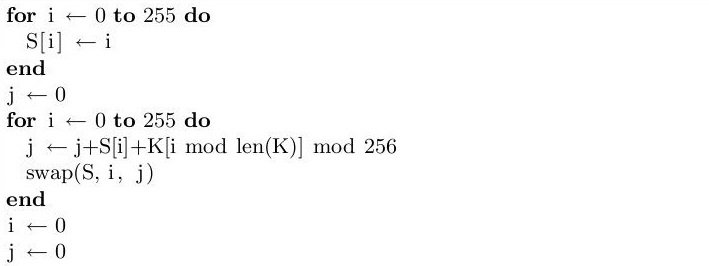
\includegraphics[width=10.5cm,height=5cm]{RC2} }
\caption{Anahtar olu�turma}
\label{2}
\end{figure}
Algoritma, 256 baytl�k bir durum tablosunu ba�latmak i�in 1 ile 256 bayt aras�nda de�i�ken uzunluk anahtar� kullan�r. Durum tablosu daha sonra �ekil \ref{3}'deki gibi sahte rasgele bayt �retimi i�in ve daha sonra �ifreli metni vermek �zere d�z metinle XOR yap�lan bir sahte rasgele ak�� olu�turmak i�in kullan�l�r. Durum tablosundaki her bir ��e en az 1 kez takas edilir. 
\begin{figure}[H]
\centering
\scalebox{1}{
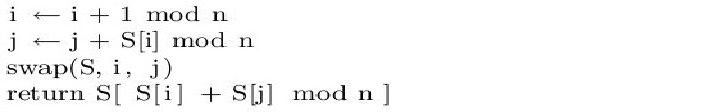
\includegraphics[width=10.5cm,height=2.5cm]{RC3} }
\caption{Anahtar ak��� olu�turma}
\label{3}
\end{figure}
\newpage 
\subsection{RC4 G��l� Y�nleri}
RC4 algoritmas�n�n g��l� y�nleri a�a��da belirtildi�i gibidir.
\begin{itemize}
\item Tabloda herhangi bir de�erin nerede oldu�unu bilmenin zorlu�u.\item Tablodaki hangi konumun dizideki her bir de�eri se�mek i�in kullan�ld���n� bilmenin zorlu�u.\item Belirli bir RC4 anahtar�n�n bir kez kullan�lmas�.\item �ifreleme DES'den 10 kat daha h�zl� olmas�.
\end{itemize}
\subsection{RC4 Kullan�m Alanlar�}
RC4; WEP, WPA gibi g�ncel bir �ok uygulamada kullan�lmaktad�r. 
\subsubsection{Wired equivalent privacy}
WEP, �ifreleme ve kimlik do�rulama i�in IEEE 802.11 taraf�ndan belirlenmi�tir. Standart, WEP'i iki ana b�l�m olarak tan�mlam��t�r. �lki kimlik do�rulama, ikincisi �ifreleme k�sm�d�r. WEP'in hedefleri �unlard�r :
\begin{itemize}
\item Do�ru WEP anahtar� bulunmad��� i�in yetkili kullan�c�lar�n eri�mesini engelleyerek ula��lan eri�im kontrol� \item Gizlilik, WLAN veri ak���n� �ifrelemek i�in WEP anahtar� kullan�larak elde edilir ve yaln�zca do�ru WEP anahtar�na sahip olanlar �ifresini ��zebilir
\end{itemize} 
\newpage
WEP taraf�ndan kullan�lan �ifreleme i�lemi Rivest Cipher 4 (RC4)'t�r. Sald�rganl�ktan ve ya yetkisiz veri de�i�ikli�inden korumak i�in kullan�lan  ICV olu�turmak i�in d�z metin �zerinde CRC-32 kullanan bir b�t�nl�k algoritmas�da vard�r. �ekil \ref{4}'de WEP'in �ifreleme algoritmas� g�sterilmi�tir. \cite{k:5}
\begin{figure}[H]
\centering
\scalebox{1}{
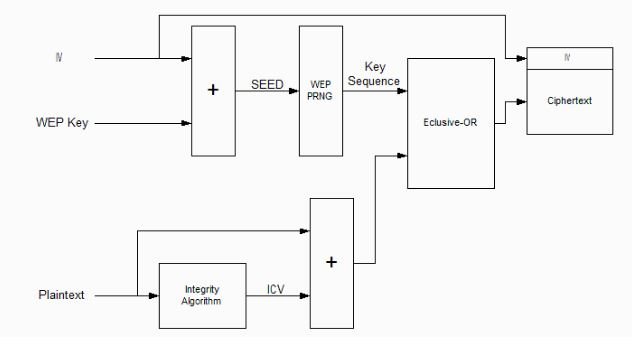
\includegraphics[width=10.5cm,height=6cm]{WEP} }
\caption{WEP �ifreleme algoritmas�}
\label{4}
\end{figure}
�ekil \ref{5}'de ise WEP �ifrelemesinin geri d�n���m algoritmas� verilmi�tir.
\begin{figure}[H]
\centering
\scalebox{1}{
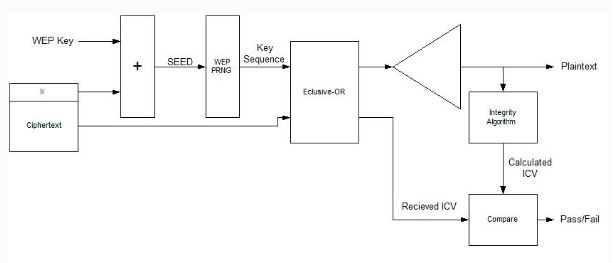
\includegraphics[width=10.5cm,height=6cm]{WEP2} }
\caption{WEP �ifreleme geri d�n���m algoritmas�}
\label{5}
\end{figure}
\newpage
\subsubsection{Wireless protected access}
IEEE 802.11'i kablosuz a� standard�, LAN'� g�venli�indeki geli�meleri belirtir. Yeni IEEE 802.11'i standard� onaylan�rken, kablosuz �r�n sat�c�lar� WPA olarak bilinen, �e�itli sistemlerin birlikte �al��mas�na olanak veren ge�ici bir standart �zerinde anla�m��t�r. Geni� �ekilde kullan�lan bu iki tip WPA standard� WEP'in zay�f y�nlerini kapatmak i�in ge�ici olarak olu�turulmu�tur. Mevcut cihazlar g�ncellenirse bu protokol� kullanabilir. G�n�m�zdeki cihazlarda deste�i eklenmi� durumdad�r. WPA'n�n WEP'e tercih edilmesinde �� �nemli sebep vard�r. Bunlar;
\begin{itemize}
\item 802.1X/EAP tabanl� kar��l�kl� as�llama sa�lamaktad�r. \item WEP'e g�re daha g��l� bir �ifreleme y�ntemi olan TKIP'i desteklemektedir. \item Veri b�t�nl��� i�in MIC y�ntemini kullanmaktad�r.
\end{itemize} 

TKIP, �ok�a tatbik edilen yeni �ifreleme protokol�d�r. TKIP'in geli�tirilmesindeki en b�y�k etken, WEP tabanl� donan�m�n�n g�venli�inin artt�r�lmas� ve g�ncellenmesidir. Genel olarak, WEP kullanan donan�mlar�n yonga setleri RC4 �ifreleme i�in donan�m deste�i sa�lad�. Donan�ma yo�un uygulanan �ifreleme ile yaz�l�m donan�m ve firmware g�ncellemeleri geri kalan�n� m�mk�n k�lm��t�r. TKIP, WEP'in temel yap�s�na ve i�lemlerine sahiptir. WEP tabanl� ��z�mlere kar��l�k bir yaz�l�m g�ncellemesi olarak tasarlanm��t�r. Esas olarak WEP kusurlu olarak g�sterildi�i i�in protokol onu WEP'ten ay�rabilmek i�in yeniden adland�rm��t�r. TKIP yukar�da belirtildi�i gibi RC4 ak�� �ifrelemesini de kullan�r. Sebebi WPA tam bir g�venlik standard� olarak geli�memi�tir. \cite{k:6} 


\section{2B CAT MAP KAOT�K S�STEM�}
Projede g�r�nt� �ifreleme i�lemi yap�l�rken, �ifrelemeden �nce se�ilen g�r�nt� MATLAB'da 2B Cat Map kullan�larak kar��t�r�lm��t�r. Kar��t�r�lan g�r�nt� daha sonra �ifrelenmek �zere programda belli i�lemlere tabii tutulmu�tur.
\subsection{2B Cat Map Nedir ? Nas�l �al���r ?}
G�r�nt� kar��t�rma perm�tasyon evresinde genellikle iki boyutlu �� tip kaotik harita kullan�lmaktad�r. Bunlar Standart Map, Cat Map ve Genelle�tirilmi� Baker Map haritalar�d�r. Cat Map literat�rde en yayg�n kullan�lan haritad�r. M x N boyutlu bir g�r�nt� ve bu g�r�nt�ye ait piksel de�erlerinin koordinatlar� C={(x,y)| x,y =1,2..,N} olarak belirlenirse Cat Map a�a��daki gibi tan�mlan�r. \cite{k:2}
\begin{figure}[H]
\centering
\scalebox{1}{
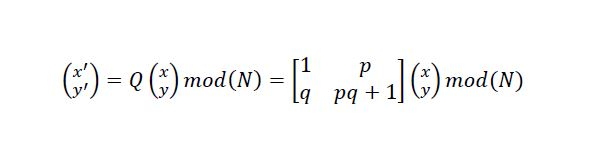
\includegraphics[width=10.5cm,height=3cm]{catmap} }
\caption{Cat map g�r�nt� kar��t�rma algoritmas�}
\label{6}
\end{figure}  
\newpage
�ekil \ref{6}'de g�sterilen denklemde Cat Map kontrol parametreleri olan p ve q pozitif tamsay�lard�r. (x,y) ve (x',y') de�erleri ise s�ras�yla koordinat de�erlerinin orjinal ve yeni pozisyonlar�d�r. Burada det(Q)=1 oldu�undan alan korunur, yani herhangi bir koordinat birbiriyle �ak��maz ve herhangi bir kay�p meydana gelmez. 
\begin{figure}[H]
\centering
\scalebox{1}{
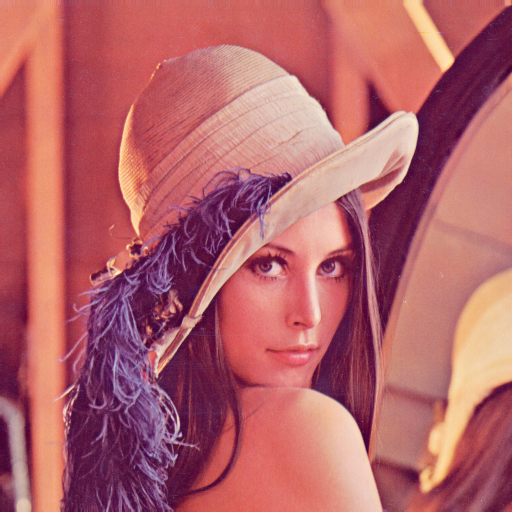
\includegraphics[width=10.5cm,height=6cm]{lena} }
\caption{Orjinal Lena g�r�nt�s�}
\end{figure}

2B Cat Map, s�n�rlar� belirli bir alanda s�rekli farkl� koordinat de�erleri �reterek g�r�nt�deki piksellerin yerlerinin de�i�imini sa�lamaktad�r. Yukar�daki �ekildeki Lena g�r�nt�s� 2B Cat Map sistemine giri� olarak uyguland���nda �ekil \ref{7}'deki gibi farkl� �ekillerde g�r�nt� pikselleri kar��t�r�labilmektedir. G�r�nt� piksellerinin kar���m�ndaki farkl�l�k 2B Cat Map sisteminde bulunan p ve q parametlerinden kaynaklanmaktad�r. �ekil \ref{7}'de elde edilen g�r�nt�lerde p=1 ve q=1 se�ildi�inde (a) g�r�nt�s�, p=5 ve q=7 se�ildi�inde (b) g�r�nt�s�, p=22 ve q=30 se�ildi�inde (c) g�r�nt�s�, p=401 ve q=401 se�ildi�inde (d) g�r�nt�s� elde edilmektedir. Bu de�erlerin de�i�iminden de anla��laca�� �zere p ve q de�erleri artt�r�ld�k�a g�r�nt�deki pikseller daha homojen kar��maktad�r. 
\newpage
\begin{figure}[H]
\centering
\scalebox{1}{
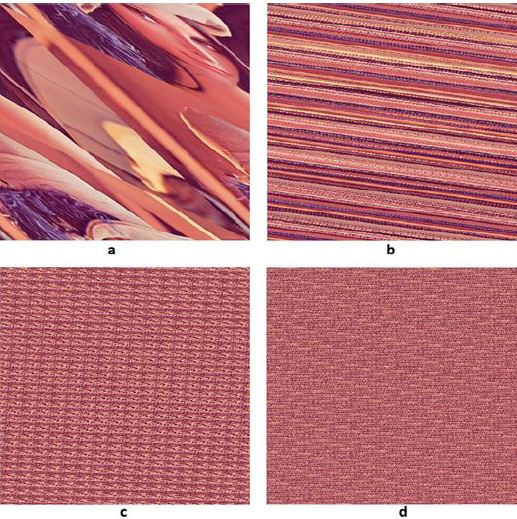
\includegraphics[width=12.5cm,height=8cm]{lena2} }
\caption{Kar��t�r�lm�� Lena g�r�nt�leri}
\label{7}
\end{figure}
Piksellerin koordinatlar�n�n de�i�mesi, g�r�nt� �ifreleme i�lemlerinde b�y�k kolayl�k sa�lamaktad�r. Orjinal g�r�nt�de bulunan biti�ik piksel de�erleri birbirine �ok yak�n olaca��ndan, bu k�s�mlar �ifrelendi�inde birbirine yak�n de�erler olu�turabilmektedir. Fakat 2B Cat Map uygulanan g�r�nt�de biti�ik piksel de�erleri farkl�la�acakt�r. Bu sayede daha sa�lam bir �ifreleme yap�labilecektir. G�r�nt� kar��t�rma i�lemleri tamamland�ktan sonra g�r�nt�n�n tekrar eski haline getirilmesi �ekil \ref{8}'deki gibi tan�mlan�r. 
\begin{figure}[H]
\centering
\scalebox{1}{
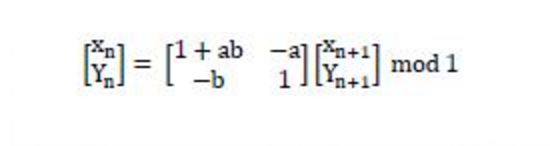
\includegraphics[width=10.5cm,height=3cm]{catmapreverse} }
\caption{2B Cat Map ile kar��t�r�lan g�r�nt�n�n geri d�n��t�r�lmesi}
\label{8}
\end{figure}
 
\section{��FRELEME ��LEMLER�}
Bu b�l�mde C\# program� ile RC4 �ifrelemesi yap�l�rken program�n sadece �ifreleme a�amalar� ve kodlar� anlat�lm��t�r. 
\subsection{RC4 S�n�f�n�n Olu�turulmas�}
�ifreleme i�lemlerine ba�lamadan �nce C\# 'da RC4 ad� verdi�imiz bir s�n�f olu�turuyoruz. Bu s�n�fta RC4 algoritmas�n�n kullan�laca�� �ifreleme i�lemleri bulunmaktad�r. RC4 s�n�f�nda kullan�lmak �zere d��ar�dan anahtar ve �ifrelenecek (ve ya geri d�nd�r�lecek) metin al�nmaktad�r. �lk olarak s�n�f�m�zda d��ar�dan al�nan bu iki de�er set ve get edilir. Daha �nce anlat�ld��� gibi RC4 algoritmas� iki farkl� a�amadan olu�maktad�r. Bu s�n�f�m�z i�inde ilk olarak sbox olu�umundan bahsedece�iz. Sbox bizim bu s�n�fta olu�turdu�umuz bir dizi olup, �ifreleme i�lemleri ger�ekle�irken bu dizi baz al�nacakt�r. Sbox girilen anahtara g�re �ekil \ref{9}'deki gibi olu�turulmaktad�r.
\begin{figure}[H]
\centering
\scalebox{1}{
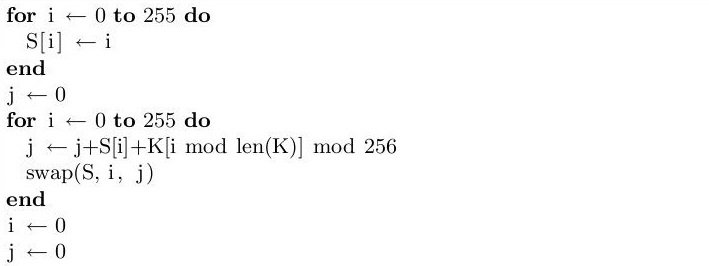
\includegraphics[width=10.5cm,height=5cm]{RC2} }
\caption{Sbox olu�umu}
\label{9}
\end{figure}
�ekil \ref{9}'de g�r�len algoritmay� a��klayacak olursak; algoritma gere�i d�ng� 256'ya kadar gitmektedir. Bunun i�in N de�i�keni, RC4 s�n�f�n�n ba��nda tan�mlanm�� olup, t�m program boyunca algoritman�n gere�i olarak sabit de�er  256 tan�mlanm��t�r. Sbox olu�umu i�in kullan�c�n�n girdi�i anahtar kelime kullan�larak yeni bir dizi olu�turulmu�tur. For d�ng�s� ile anahtar�n harflarinin int tipindeki de�erleri, anahtar kelimenin uzunlu�uyla mod al�narak 256 boyutlu bir yeni dizi olu�turmaktad�r. Ayn� for d�ng�s� i�inde sbox'da olu�turulmaktad�r. Di�er for d�ng�s�nde yine 256'ya kadar algoritma gere�i ilk olarak 0 olarak tan�mlanan b de�eri, sbox de�eri ve yeni dizinin de�erleri toplanarak de�i�tirme i�lemleri uygulan�r. B�ylelikle ilk olarak 1'den ba�lay�p 256'ya kadar de�er alan sbox yeni de�erlerini alm�� olur. B�ylelikle iki a�amadan meydana gelen RC4'�n ilk a�amas� tamamlanm�� olur.

RC4'�n algoritmas�nda bulunan ikinci a�ama ise Sifrele() metodu ile tan�mlanm��t�r. ilk a�amada �retilen sbox Sifrele() metodunun en ba��nda �a��r�l�r ve �e�itli i�lemler ile �ekil \ref{10}'deki algoritmadaki gibi kullan�l�r. 

\begin{figure}[H]
\centering
\scalebox{1}{
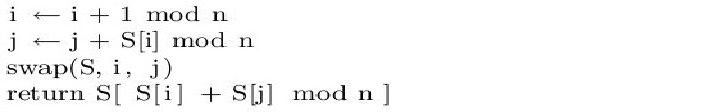
\includegraphics[width=10.5cm,height=2.5cm]{RC3} }
\caption{�ifreleme a�amas�}
\label{10}
\end{figure}
�ekil \ref{10}'deki algorima Sifrele() metodu ile birlikte kullan�l�rken i�lem kolayl��� ve performans a��s�ndan StringBuilder s�n�f� kullan�lm��t�r. RC4 algoritmas�n�n genel yap�s�nda bulunan gerekliliklerden �t�r� yukar�da da g�r�ld��� gibi baz� mod alma i�lemleri ve yer de�i�tirme i�lemleri uygulanm��t�r. En sonda olu�turulan  de�er ile �ifrelenecek ve ya geri d�nd�relecek metod XOR i�lemine girer. B�ylelikle �ifrelenmeden �nceki son a�ama olan bu a�amada d�n��t�r�lmeden �nce �ifrelenmi� de�erler belirlenmi� olur.

RC4 s�n�f�nda StrToHexStr ve HexStrToStr olmak �zere iki metod daha bulunmaktad�r. Fakat bu metodlar form ekran�ndaki butonlara t�kland�k�a kullan�laca�� i�in daha sonra bahsedilecektir. 
\newpage
\subsection{Form Ekran�n�n Tasarlanmas�}
Bu b�l�mde form ekran�nda bulunan Toolbox'lar�n neler oldu�u, ne ama�la form ekran�nda bulunduklar� ve form ekran�ndaki yerle�imleri hakk�nda bilgi verilecektir. �ncelikle, form ekran�nda bulunan Toolbox'lar a�a��daki gibidir:
\begin{itemize}
\item Buton \item OpenFileDialog \item SaveFileDialog \item Label \item PictureBox \item TextBox
\end{itemize}
\subsubsection{Buton kullan�m�}
Form ekran�nda birden fazla buton kullan�lm��t�r. Kullan�lan bu butonlar �ifrelenecek belgeyi se�mede, se�ilen belgeyi �ifrelemede, �ifrelenen belgeyi geri se�mede, se�ilen belgeyi geri d�nd�rmede ve kay�t i�lemlerinde kullan�lmaktad�r.
\subsubsection{OpenFileDialog kullan�m�}
OpenFileDialog kullan�m� �ifrelenecek belgeyi se�mek i�in pencere a��lmas�nda ve kay�t i�lemlerinde kay�t yerinin belirlenmesi i�in pencere a��lmas�nda kullan�lmaktad�r.
\subsubsection{SaveFileDialog kullan�m�}
SaveFileDialog ad�n�n T�rk�e kar��l���ndanda anla��laca�� gibi kay�t i�lemlerinin yap�lmas� i�in gereklidir. �ifrelenen metni belge haline d�n��t�r�p kaydetme i�leminde ve �ifrelenmi� metinin geri d�nd�r�l�p as�l haline ula�t�ktan sonra kay�t etme i�levlerinde kullan�lmaktad�r.
\subsubsection{Label kullan�m�}
Form ekran�nda gerekli g�r�len yerlere ba�l�k eklemek i�in kullan�lmaktad�r.
\subsubsection{PictureBox kullan�m�}
Form ekran�nda �ifrelenecek belgeyi se�erken, se�ilen belgenin bir g�r�nt� olmas� halinde pictureBox ekran�nda g�r�nt�lenmesi i�in kullan�lmaktad�r.
\subsubsection{TextBox kullan�m�}
Form ekran�nda kullan�c� taraf�ndan girilecek olan anahtar kelimeyi yazmada, gerek belge olarak, gerekse kullan�c� taraf�ndan �ifrelenecek bir metin girilmesi i�in ve �ifrelenmi� metnin g�r�nt�lenmesi i�in kullan�lmaktad�r.
\newpage
T�m bu Toolbox'lar�n kullan�m� sonucunda form ekran� �ekil \ref{11}'deki gibi  meydana gelmi�tir.
\begin{figure}[H]
\centering
\scalebox{1}{
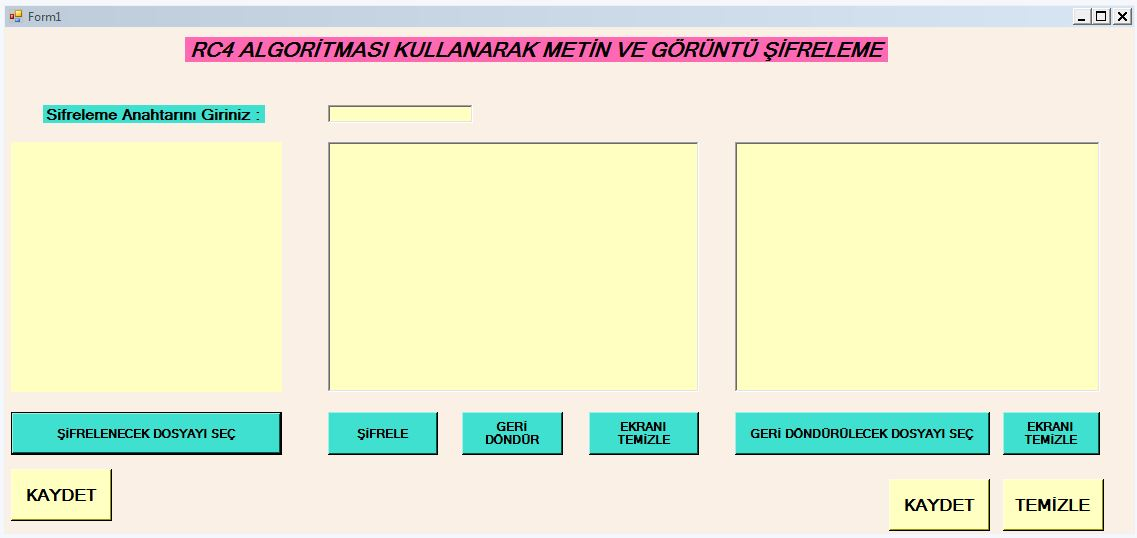
\includegraphics[width=10.5cm,height=6cm]{form} }
\caption{Form ekran�}
\label{11}
\end{figure}
\subsection{�ifreleme ��lemi}
RC4 s�n�f�n�n ve form ekran�n�n olu�umundan sonra �ifreleme i�in gerekli kodlar�n yaz�lmas�nda bir engel kalmam��t�r. �lk  olarak �ifreleme yapabilmek i�in e�er klavyeden bir metin girilerek �ifreleme yap�lmak istenmiyorsa �ifreleme yapabilmek i�in bir dosya se�ilmelidir. Bu dosyay� se�mek i�in form ekran�nda bir buton olu�turulmu�tur. ��FRELENECEK DOSYAYI SE� butonu ile �ifrelenmesi istenen dosya �ekil \ref{12}'de g�sterildi�i gibi se�ilmektedir.
\begin{figure}[H]
\centering
\scalebox{1}{
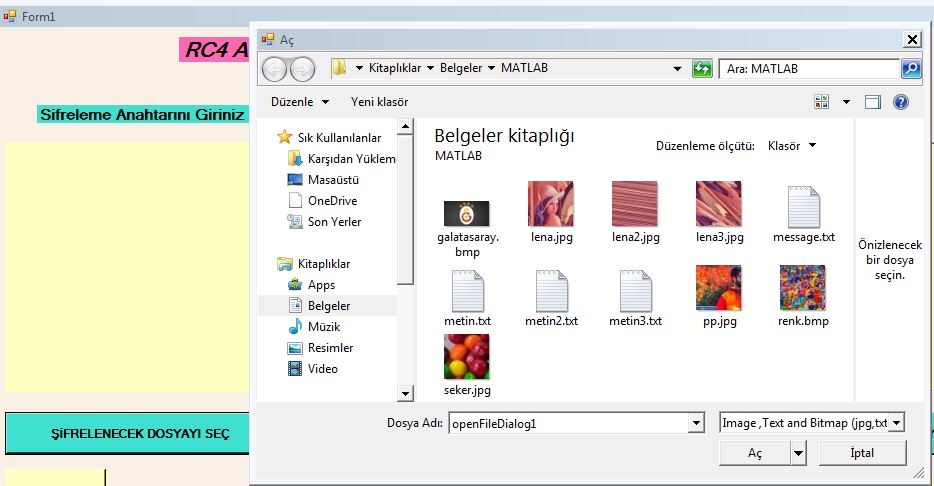
\includegraphics[width=10.5cm,height=6cm]{filedialog} }
\caption{�ifrelenecek dosyan�n se�ilmesi}
\label{12}
\end{figure}
\newpage
Bu se�im i�lemi OpenFileDialog kullan�larak ger�ekle�tirilmektedir. Dosya se�ilirken metin ve g�r�nt� �ifrelemesi yap�laca��ndan �t�r� ��kan sonu�lar filtrelenmi�tir. Sadece .jpg, .bmp ve .txt dosyalar� g�r�nt�lenecektir. Try catch yap�s� kullan�larak se�ilen dosyan�n metin ve ya g�r�nt� olmas�na g�re ayr� ayr� yap�lacak i�lemler belirlenmi�tir. E�er se�ilen belge bir g�r�nt� ise bu g�r�nt�n�n �ifrelenebilmesi i�in byte tipine d�n��t�r�lmesi gerekmektedir. Bunun i�in se�ilen g�r�nt� ImageToBase64 metoduna g�nderilerek g�r�nt�n�n byte tipine �evrilmesi sa�lan�r. Ard�ndan byte tipine �evrildikten sonra de�erler �ifrelenmek i�in �ifreleme textBox'�na  yazd�r�l�r. G�r�nt�n�n �ifrelenmeden �nce g�nderildi�i ImageToBase64 metodu �ekil \ref{13}'deki gibi verilmi�tir. \cite{k:7}
\begin{figure}[H]
\centering
\scalebox{1}{
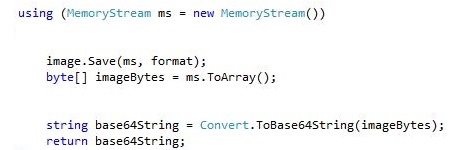
\includegraphics[width=10.5cm,height=4cm]{tobase64} }
\caption{ImageToBase64 metodu}
\label{13}
\end{figure} 
MemoryStream s�n�f� kullan�larak yap�lan bu d�n���m sonucunda string tipinde ��kan sonu� �ifrelemenin yap�laca�� textBox'a yazd�r�l�r. Bu a�amadan sonra �ifreleme yapabilmek i�in ��FRELE butonu devreye girer.
\newpage
Form ekran�nda bulunan ��FRELE butonuna basarak �ifreleme i�lemi ba�lar. Butona t�klad�ktan sonra �ekil \ref{14}'de �ifreleme ekran�ndaki metin �ifrelenerek �ifrelenmi� alana yazd�r�l�r. 
\begin{figure}[H]
\centering
\scalebox{1}{
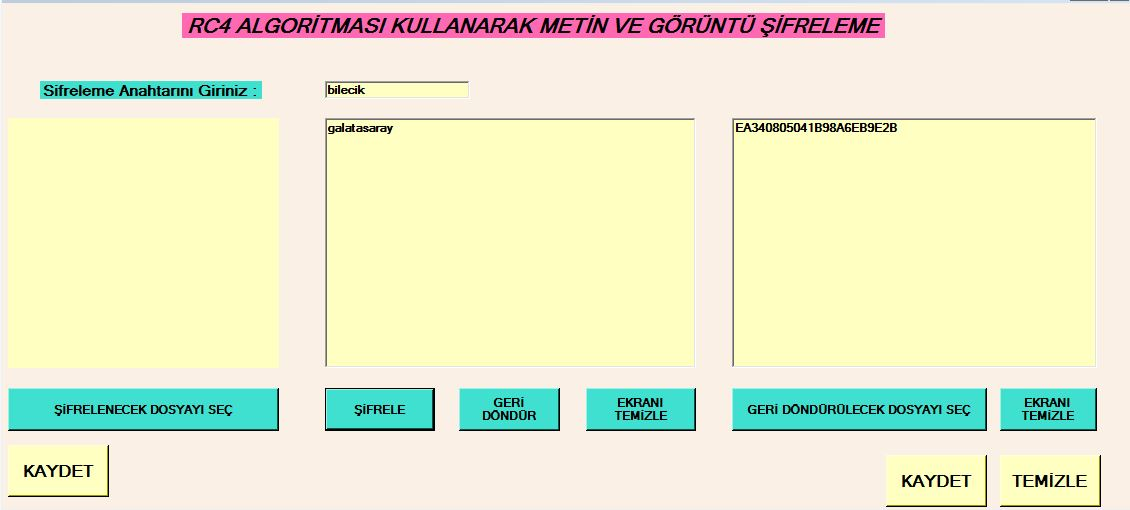
\includegraphics[width=13.5cm,height=8cm]{sifrelebuton} }
\caption{�ifreleme i�lemi}
\label{14}
\end{figure}
��FRELE butonunun i�inde bulundurdu�u kodda �ncelikle kullan�c� taraf�ndan girilmesi zorunlu olan anahtar�n girilip girilmedi�i kontrol edilir. E�er bu alan bo� b�rak�lm�� ise Message.Show ile bir hata mesaj� g�sterilir ve �ifreleme anahtar�n�n bo� ge�ilemeyece�i bildirilir. E�er �ifreleme anahtar� olmas� gerekti�i gibi girilmi� ise �ncelikle RC4 s�n�f�ndan bir nesne olu�turulur ve bu s�n�fa girilen �ifreleme anahtar� ve �ifrelenmek i�in olu�turulan TextBox'daki metin g�nderilir. RC4 s�n�f�nda meydana gelen i�lemler sonucunda ��kan sonu� Hex tipine �evrilmek �zere StrToHexStr metoduna g�nderilir ve �evrilen de�er �ifreli metinin g�sterilmesi i�in olu�turulan TextBox'a yans�t�l�r.

�ifrelenmek �zere g�nderilen metin farkl� tiplerde yans�t�labilir. Fakat yap�lan ara�t�rma sonucu en yayg�n kullan�m� Hex tipi oldu�undan burada �ifreli metin Hex tipinde g�sterilmi�tir. Hex tipine �evirme i�lemi �ekil \ref{15}'de g�sterildi�i gibidir.
\newpage
\begin{figure}[H]
\centering
\scalebox{1}{
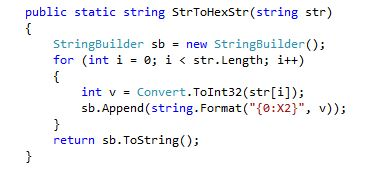
\includegraphics[width=10.5cm,height=3.8cm]{strtohex} }
\caption{�ifrelenen metinin stringden hex tipine d�n���m�}
\label{15}
\end{figure}  
Bu d�n���m i�lemi yap�l�rken yine kolayl�k ve performans a��s�ndan StringBuildir s�n�f� kullan�lm��t�r. Burada g�nderilen metin int tipine �evrildikten sonra StringBuilder s�n�f�na ait string.Format metodu ile hex tipinde g�sterilmi�tir. string.Format metodu farkl� bir tipteki de�i�keni ba�ka bir tipte g�stermeye yarar. Nitekim burada int tipindeki her bir de�eri 2 haneli hex de�erler olarak g�sterilmi�tir. \cite{k:8}

B�ylelikle �ifreleme i�lemi tamamlanm�� olur. En ba��ndan beri konuyu ele al�p �zetleyecek olursak, �ifrelenenmek �zere belge se�ildikten sonra se�ilen belge g�r�nt� ise �nce byte tipine �evrildi ve daha sonra �ifrelenmek �zere textBox'a yazd�r�ld�. Ayn� zamanda �ifreleme i�in �ifreleme anahtar�n�n girilmesi sa�land�. E�er se�ilen dosya metin belgesi ise se�ilen metin belgesi textBox'a yazd�r�ld�. TextBox'daki bu de�erler hex tipine �evrilerek �ifrelenmi� alanda bulunan textBox'a yazd�r�ld� ve �ifreleme i�lemi tamamlanm�� oldu. 
\subsection{�ifreli Metinin Kaydedilmesi}
�ifreleme i�lemleri tamamland�ktan sonra form ekran�nda bulunan iki KAYDET butonundan sa� alttaki ile �ifreli metin kaydedilebilmektedir. Kay�t edilen bu �ifreli metin daha sonra geri d�nd�r�lmek �zere kullan�lacakt�r.
\newpage
\section{GER� D�ND�RME ��LEMLER�}
Bu b�l�mde RC4 ile �ifrelenen �ifreli metni tekrar eski haline d�nd�rme i�lemlerinden bahsedilecektir.
\subsection{Kaydedilen �ifreli Metinin Se�ilmesi}
�ifreleme i�lemleri tamamland�ktan sonra �ifreli metin KAYDET butonu ile kaydedildi. Geri d�nd�rme i�lemi yap�l�rken form ekran�nda bulunan GER� D�ND�R�LECEK DOSYAYI SE� butonu ile �ifrelenmi� metin OpenFileDialog ile se�ilerek �ifrelenmi� metin form ekran�na yans�t�l�r. Bu yans�tma i�lemi StreamReader s�n�f� ile �ekil \ref{16}'de g�sterildi�i gibi ger�ekle�mektedir. 
\begin{figure}[H]
\centering
\scalebox{1}{
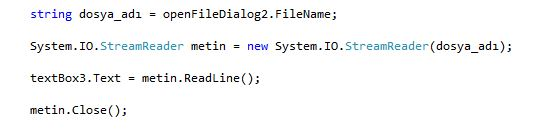
\includegraphics[width=10.5cm,height=3.5cm]{stream} }
\caption{StreamReader s�n�f�n�n kullan�m�}
\label{16}
\end{figure} 
�ekil \ref{16}'de g�r�len StreamReader s�n�f� OpenFileDialog ile se�ilen metni okur ve form ekran�nda belirtilen yere yazar. Bu a�amadan sonra geri d�nd�r�lmesi istenen form ekran�na gelmi�tir. Art�k GER� D�ND�R butonu ile �ifreli metin ilk haline d�n��t�r�lecektir. 
\subsection{Geri D�nd�rme ��lemi}
�ifrelenen metin geri d�nd�r�lmek �zere se�ildikten sonra geri d�nd�rme i�leminin yap�labilmesi i�in girilen anahtar kelimenin �ifreleme yap�l�rken kullan�lan anahtar kelime ile e�de�er olmas� gerekmektedir. Aksi taktirde �ifreli metin yeni anahtar kelimeye g�re d�nd�r�lecektir ve bu da olumsuz sonu� al�nmas�na neden olacakt�r. 

Geri d�nd�rme i�lemi yap�l�rken �ifreli metin hex tipinde bir metindi. �ncelikle hex tipindeki metinin stringe �evrilmesi gerekmektedir. Bunun i�in HexStrToStr metodu �ekil \ref{17}'de g�sterildi�i gibi kullan�lm��t�r. \cite{k:9}
\begin{figure}[H]
\centering
\scalebox{1}{
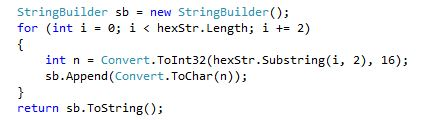
\includegraphics[width=10.5cm,height=3.5cm]{hextostr} }
\caption{HexStrToStr metodunun kullan�m�}
\label{17}
\end{figure}

�ekil \ref{17}'de g�sterilen metod sayesinde hex tipinde �ifrelenmi� olan �ifreli metin string tipine d�n��t�r�l�r. B�ylelikle geri d�nd�rme i�lemi i�in son bir a�ama kalm�� olur. String t�r�ne �evrilen metin RC4 s�n�f�na girilen anahtar kelime ile tekrar g�nderilir ve  i�lemler sonucunda XOR'lanarak eski haline d�n��t�r�lm�� olur. D�n��t�r�len bu d�z metin try catch ile iki farkl� durum i�in incelenmektedir. E�er �ifreleme yap�lan dosya bir metin ise geri d�nd�rme i�lemleri sonucunda o metin form ekran�nda belirtilen yere yazd�r�lacakt�r. Ama e�er �ifrelenmesi i�in se�ilen dosya bir g�r�nt� ise geri d�nd�r�len metin Base64ToImage metodu ile tekrar bir g�r�nt� haline getirilir ve form ekran�nda bulunan pictureBox'ta g�sterilir. B�ylelikle se�ilmesi muhtemel iki durum i�inde geri d�nd�rme i�lemleri tamamlanm�� olur. 

Geri d�nd�rme i�lemleri tamamland�ktan sonra form ekran�nda g�sterilen daha �nce 2B Cat Map ile kar��t�r�lm�� g�r�nt�, form ekran�n�n sol alt k�sm�nda bulunan KAYDET butonu ile tekrar kar��t�r�l�p eski haline getirilmesi i�in kaydedilmektedir. 

\section{SONU�LAR VE �NER�LER}
Sonu� olarak bu projede RC4 algoritmas� kullan�larak metin ve g�r�nt� �ifrelemesi C\# programlama dili yard�m� ile �ifrelenmi� ve daha sonra geri d�nd�r�lm��t�r. G�r�nt� �ifrelemesi yapmadan �nce ise MATLAB yard�m� ile 2B Cat Map Kaotik Sistemi kullan�larak g�r�nt� kar��t�r�lm�� ve �ifrelenme i�leminden sonra geri d�nd�rme i�lemide uyguland�ktan sonra tekrar Cat Map ile kar��t�r�lan g�r�nt� eski haline d�n��t�r�lm��t�r. �ekil \ref{18}'de program�n son hali g�sterilmi�tir. Burada se�ilen g�r�nt� daha anla��l�r olmas� a��s�ndan Cat Map ile kar��t�r�lmadan �ifrelenmi�tir. 
\begin{figure}[H]
\centering
\scalebox{1}{
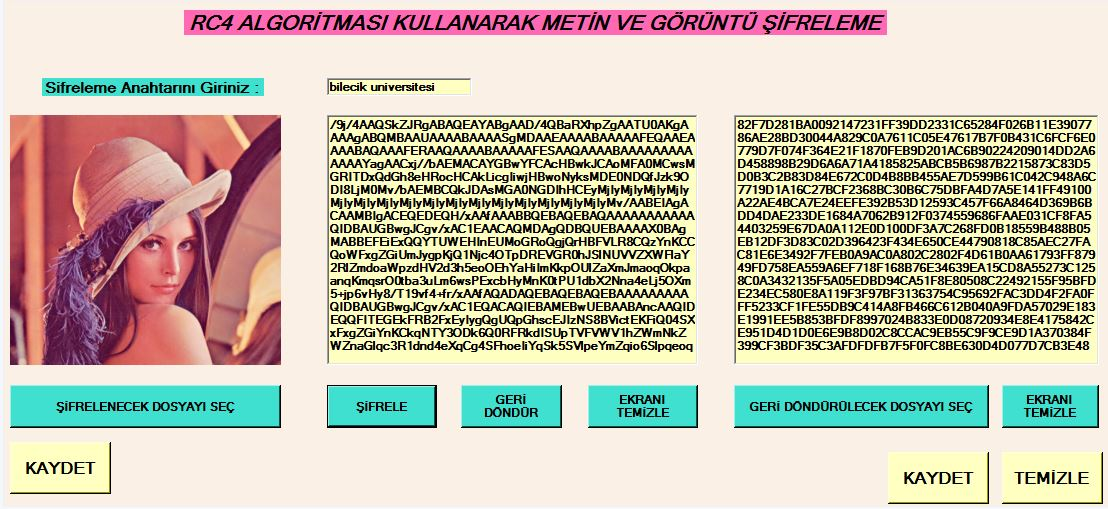
\includegraphics[width=14.5cm,height=10cm]{sonuc}}
\caption{Lena g�r�nt�s�n�n RC4 ile �ifrelenmesi}
\label{18}
\end{figure}

RC4 algoritmas�nda �ifrelenecek dosyalar �e�itli Kaotik Sistemler kullan�larak �ifreleme i�lemi ��z�lmesi daha g�� bir hale getirilebilir. \ref{sonuc}
\section{EKLER}
Bu proje s�recinde, proje konusuna dahil olmayan Runge Kutta y�nteminin MATLAB ortam�nda uygulamas� yap�lm��t�r. Runge Kutta y�ntemi EK-1'de, rapor i�erisinde konusu ve uygulamas� ge�en fakat i�eri�indeki kod k�sm� hakk�nda �ok fazla bilgi verilmeyen MATLAB ortam�nda Cat Map ile g�r�nt� kar��t�rma uygulamas�n�n kodu EK-2'de verilmi�tir.

\subsection{EK-1}
Say�sal analizde Runge Kutta y�ntemleri, adi diferansiyel denklemlerin ��z�m yakla��mlar� i�in a��k yinelemeli y�ntemler ailesinin �nemli bir tipidir. Bu y�ntem 1900'l� y�llarda C. Runge ve M. W. Kutta adl� matematik�iler taraf�ndan geli�tirilmi�tir. 4. dereceden klasik Runge Kutta y�ntemi RK4 veya Runge-Kutta y�ntemi olarak adland�r�l�r. Bu y�ntem s�k�a kullan�l�r. 4. dereceden Runge Kutta y�ntemi a�a��daki �ekil \ref{25}'de g�sterildi�i gibi tan�mlan�r.

\begin{figure}[H]
\centering
\scalebox{1}{
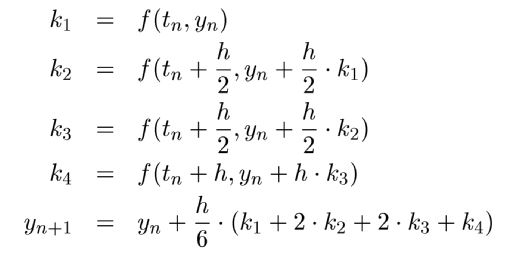
\includegraphics[width=10.5cm,height=4cm]{runge2} }
\caption{Runge Kutta y�ntemi}
\label{25}
\end{figure}
\newpage
B�ylece bir sonraki de�er, o anki de�erine ve aral���n b�y�kl���yle tahmini e�imin �arp�m�n�n eklenmesiyle elde edilir. Bu e�im, e�imlerin a��rl�kl� ortalamas�d�r. 
\begin{itemize}
\item[\textbf{k1}] aral���n ba�lang�c�ndaki e�imdir. 
\item[\textbf{k2}] aral���n orta noktas�ndaki e�imdir. 
\item[\textbf{k3}] yine orta noktadaki e�imdir. Ancak \textbf{k2} e�iminden elde edilir. 
\item[\textbf{k4}] aral���n sonundaki e�imdir ve \textbf{k3} e�iminden yararlan�larak bulunur.
\end{itemize}

Runge Kutta y�nteminin MATLAB kodu �ekil \ref{26}'de, ekran ��kt�s� ise �ekil \ref{27}'de g�sterilmi�tir.
\begin{figure}[H]
\centering
\scalebox{1}{
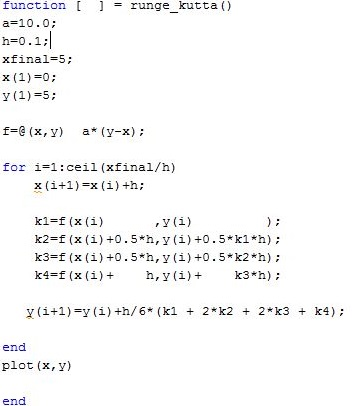
\includegraphics[width=10.5cm,height=8cm]{runge} }
\caption{Runge Kutta y�ntemi MATLAB kodu}
\label{26}
\end{figure}
\newpage
\begin{figure}[H]
\centering
\scalebox{1}{
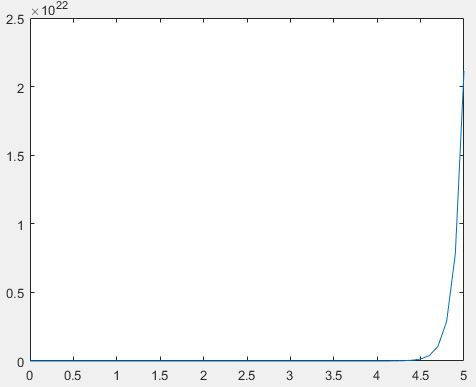
\includegraphics[width=10.5cm,height=6cm]{runge3} }
\caption{Runge Kutta y�ntemi ekran ��kt�s�}
\label{27}
\end{figure}

\subsection{EK-2}
MATLAB ile 2B Cat Map g�r�nr� kar��t�rma ve g�r�nt�y� geri d�nd�rme kodlar� a�a��da �ekil \ref{28} ve �ekil \ref{29}'de verilmi�tir.

\begin{figure}[H]
\centering
\scalebox{1}{
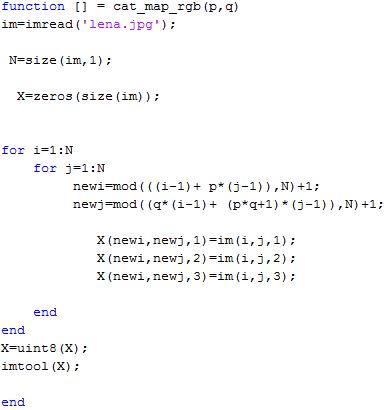
\includegraphics[width=10.5cm,height=8cm]{catmaprgb} }
\caption{2B Cat Map ile g�r�nt� kar��t�rma}
\label{28}
\end{figure}

\begin{figure}[H]
\centering
\scalebox{1}{
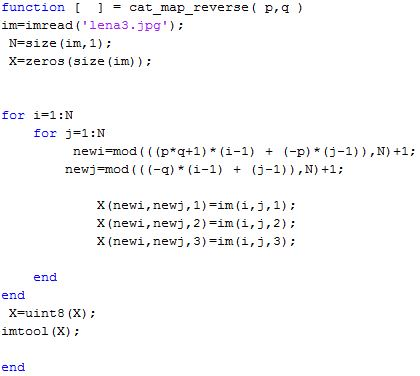
\includegraphics[width=10.5cm,height=8cm]{catmaprgbreverse} }
\caption{2B Cat Map ile kar��t�r�lan g�r�nt�n�n reverse edilmesi}
\label{29}
\end{figure}
%kaynaklar ba�l���n� tan�mlar
\renewcommand{\refname}{KAYNAKLAR}

\addcontentsline{toc}{section}{KAYNAKLAR}
\begin{thebibliography}{99}%kaynak ortam� olu�turmak i�in
%%%%%%%%%%%%Kaynak Web sayfas�ndan al�nm�� ise%%%%%%%%%%%%%%%%%
\bibitem{k:1} Wikipedia, \url{https://en.wikipedia.org/wiki/RC4} 

\bibitem{k:2} Ulusal Tez Merkezi, Ar�. G�r. Sefa TUN�ER Kaotik Sistemler Tezi
\bibitem{k:3} \url{http://www.teknokolikler.com/2011/11/c-nedir-c-temelleri-nelerdir.html}
 
\bibitem{k:4} \url{http://www.teknokoliker.com/2011/11/c-nedir-c-temelleri-nelerdir.html}
\bibitem{k:5} \url{https://www.vocal.com/secure-communication/wired-equivalent-privacy-wep/}
\bibitem{k:6} \url{http://www.emo.org.tr/ekler/7600d163fa81512_ek.pdf}
\bibitem{k:7} \url{https://stackoverflow.com/questions/21325661/convert-image-path-to-base64-string}
\bibitem{k:8} Microsoft, \url{https://social.msdn.microsoft.com/Forums/en-US/74fdc1b9-9074-4c49-b90d-fbd1947c2e00/string-to-hexadecimal?forum=Vsexpressvcs} 
\bibitem{k:9} Microsoft, \url{https://msdn.microsoft.com/tr-tr/library/aka44szs(v=vs.110).aspx}

\end{thebibliography}
\centerline{\textbf{�ZGE�M��}}
\addcontentsline{toc}{section}{�ZGE�M��}
\begin{table}[H]
{
\renewcommand{\arraystretch}{1.5}
\begin{tabular}{l@{\bf :}l}
\multicolumn{2}{l}{\underline{\bf K���SEL B�LG�LER}}\cr
\textbf{Ad� Soyad�} &\hspace{0.1cm} F�rat U�AR    \cr
\textbf{Uyru�u}&\; TC  \cr
\textbf{Do�um Yeri ve Tarihi}&\; Sultanbeyli 10.08.1994     \cr
\textbf{Adres}&\; Hamidiye mah. Balc� sok. No:6 �ekmek�y/�stanbul     \cr
\multicolumn{1}{l}{}&      \cr
\textbf{Telefon}&\;  05077687574   \cr
\textbf{e-mail}&\; firatucar94@gmail.com  \cr
\multicolumn{1}{l}{}&\cr
\multicolumn{2}{l}{\underline{\bf E��T�M DURUMU}}\cr
\textbf{Lisans ��renimi}&\; B�E� Bilgisayar M�hendisli�i B�l�m�\cr
\textbf{Bitirme Y�l�}&\; 2017-2018    \cr
\textbf{Lise}& \; Alt�nay Anadolu Lisesi   \cr
\multicolumn{1}{l}{}&\cr
\multicolumn{2}{l}{\underline{\bf �� DENEY�MLER�}}\cr
\textbf{Y�l}&\;\hspace{0.1cm}2015-2016     \cr
\textbf{Kurum}& \; Mutfark Teras Cafe - Optimal Ormanc�l�k   \cr
\textbf{Stajlar}&\; KO� Sistem - Bilecik �eyh Edebali �niversitesi Bilgisayar M�hendisli�i     \cr
\multicolumn{1}{l}{}&\cr
\underline{\textbf{YABANCI D�LLER:}}&\; Spor, m�zik \cr
\multicolumn{1}{l}{}&\cr
\underline{\textbf{YABANCI D�LLER:}}&\; �ngilizce \cr  
\multicolumn{1}{l}{}&\cr
%\multicolumn{2}{l}{\underline{\bf BEL�RTMEK �STED���N�Z D��ER �ZELL�KLER:}}
\end{tabular}}
\end{table}
\shorthandon{=}
\end{document}
%%%%%%%%%%%%%%%%%%%%%%%%%%%B�TT�%%%%%%%%%%%%%%%%%%%%%%%%%%%%%%%%%%%%%%%%%%%%%